\section{Problema I: Bactracking}

%El pseudocodigo de enviar tipos esta muy hablado (lo cual no tengo idea si siquiera es posible escribirlo de otra forma)
%En el primer grafico de tiempos, no se dice en que unidad de tiempo esta medido. En el segundo grafico tmb
%Falta explicar los experimentos y decir que sucede en ellos
%Faltan los test para corroborar correctitud del algoritmo (ejemplos de resultados del algoritmo para mostrar que funcionan)
\subsection{Introducción}
Vamos a utilizar un algoritmo de backtraking que, en el peor caso debería decorrer todas las ramas del arbol de soluciones. Dicha complegidad será exponencial debido a que cada
valor  tiene tres posibilidades, ser pintado de rojo, azul o no ser pintado.


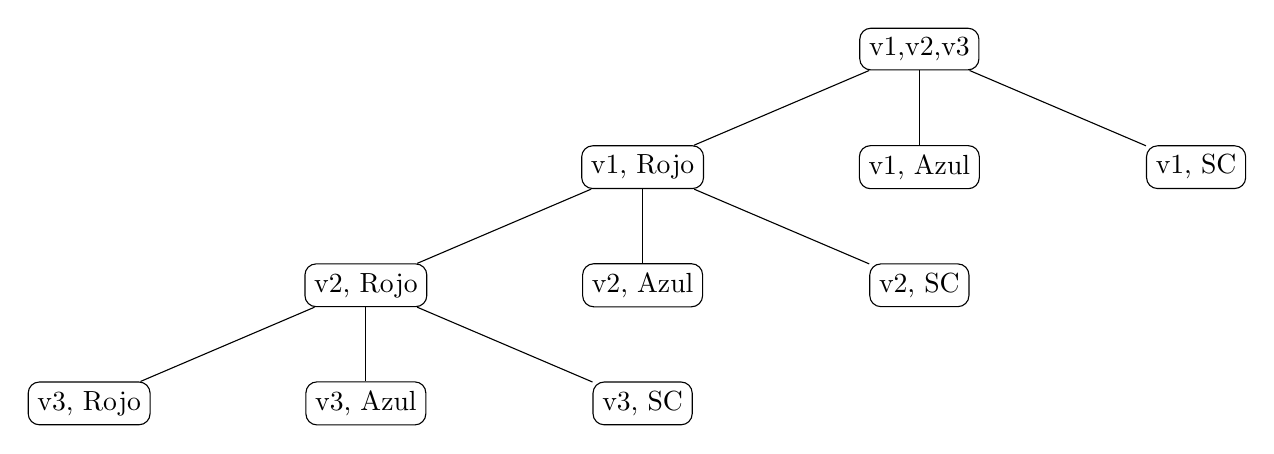
\begin{tikzpicture}[sibling distance=10em,
  every node/.style = {shape=rectangle, rounded corners,
    draw, align=center,
    top color=white, bottom color=white}]]
  \node {v1,v2,v3}
    child { node {v1, Rojo}
        child{ node {v2, Rojo}
            child{ node {v3, Rojo}}
            child{ node {v3, Azul}}
            child{ node {v3, SC}}}
        child{ node {v2, Azul}}
        child{ node {v2, SC}}}
    child { node {v1, Azul}}
    child { node {v1, SC}
 };
\end{tikzpicture}
\vspace*{5mm}

Cada yba de las hojas ultimas hojas del arbol son las posibles soluciones. En particular este arbol al tener 3 hijos va a tener 3 a la n soluciones.
\vspace*{5mm}


\subsection{Resolución del problema y representación}
Para resolver este problema con backtracing, se iterará en toda la lista substecuencias de tamaño 1 hasta el tamaño total de la secuencia
buscando la combinación maxima de elementos rojos y azules pintados. Para realizarlo presentaré el siguiente algoritmo.


Dicho  algoritmo tine como representacion dos vectores uno de enteros no negativos llamado elementos, otro de booleanos llamado validar y dos pilas una roja y otra azul con las siguientes caracteristicas:
\begin{itemize}
    \item Los elementos de las pilas son las posiciones de los elementos de las secuencias.
    \item Una pila es estrictamente creciente y la otra decreciente.
    \item Las pilas son disyuntas entre si.
    \item Todos los elementos de las pilas estan en elementos.
    \item Cuando un elemento ingresa a una pila, se asigna false a la posición de validar del elemento que ingreso.
    \item el vector validad me permite saber que elemento puedo agregar a la pila.
\end{itemize}

\subsection{Algoritmo}


El algoritmo consta de las siguientes funciones:

La función rojos se encarga de encontrar la subsecuencia maxima entre 0 e i, luego la funcion azules hace lo mismo pero siempre entre 0 y n
cada vez que un elemento es agregado a rojos o a azules, el vector validar se establece en falso para dicha posicion.



Podemos observar por medio de los ejemplos que no hay una forma clara de resolverlo sin utilizar este método: minimizar el tiempo de las idas sirve en el ejemplo 1 pero no en el ejemplo 2.
Minimizar el tiempo de las vueltas funciona para el ejemplo 2 pero no para el 1.
También podemos notar que no hay un principio de optimalidad claro: el estado 3 de menor tiempo se consigue siguiendo los pasos del ejemplo 1, pero el ejemplo 2 requiere otro estado 3 para dar el resultado óptimo.

\vspace*{5mm}

Nuestra solución primero verifica que no haya más caníbales que arqueólogos, de haber algún arqueólogo.
En ese caso, ya en el estado inicial los caníbales se los comerían.

Luego se arma el puente que cuenta con 2 objetos ``orilla'' y métodos para mover arqueólogos y caníbales de una orilla a la otra. Las orillas contienen una lista de arqueólogos y una de caníbales.

\begin{algorithm}[H]
\caption{resolver}
\begin{algorithmic}[1]
  \Procedure{resolver}{\texttt{List<Long>} arq, \texttt{List<Long>} can} $\to $ \texttt{long}
    \State \textbf{//Verifico si no hay solución.}

    \If {arq.size() $<$ can.size() $\land$ arq.size() $>$ 0}
		\State	return -1;
	\EndIf

	\State	tTotal $\gets$ $\infty$;

	\State	Orilla origen $\gets$ new Orilla(arq, can);	\State \textbf{//orilla con todos al comienzo}

	\State	Orilla destino $\gets$ new Orilla();
	\State \textbf{	//orilla destino}

	\State	Puente puente $\gets$ new Puente(origen, destino)

	\State	estados $\gets$ new ArbolEstados(arq.size(),can.size());

	\State	res $\gets$ Ida(puente, 0);

	\State return res

 \EndProcedure
\end{algorithmic}
\underline{Complejidad:} $\mathcal{O}(N+M) + \mathcal{O}(ida)$

\vspace*{5mm}
\end{algorithm}

Como recorrer una rama del árbol de backtracking es equivalente a moverse de un estado a otro inmediato (enviando una sola vez gente por el puente), y siendo que se pueden tanto enviar como recibir hasta 2 personas, los estados pueden repetirse.

Para eso creamos un árbol de estados, el cual tiene N+1 nodos representando cada uno la cantidad de arqueólogos que tiene una orilla, y cada uno de estos nodos tiene M+1 nodos hijos, representando la cantidad de can\'ibales en la misma orilla.
Cada nodo de can\'ibales posee una lista con todos los estados donde la orilla guardada tiene la cantidad de arqueólogos y caníbales correspondientes a la rama.
\\

La estructura de \'arbol es muy \'util en \'esta situaci\'on ya que permite conseguir la lista de los estados con la cantidad de arque\'ologos y can\'ibales del estado buscado, acotando la b\'usqueda significativamente.

\vspace*{5mm}
\begin{center}
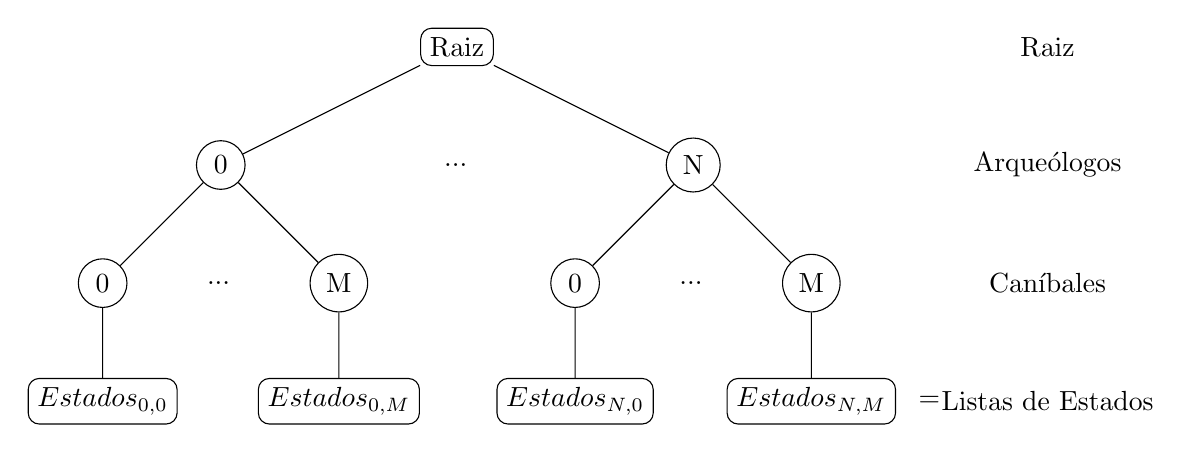
\begin{tikzpicture}[level/.style={sibling distance=60mm/#1}][H]
\node [rectangle, rounded corners, draw] (z){Raiz}
  child {node [circle,draw] (a) {0}
    child {node [circle,draw] (b) {0}
        child {node [rectangle, rounded corners, draw] (c) {$Estados_{0,0}$}}
    }
    child {node [circle,draw] (d) {M}
        child {node [rectangle, rounded corners, draw] (e) {$Estados_{0,M}$}}
    }
  }
  child {node [circle,draw] (f) {N}
    child {node [circle,draw] (g) {0}
        child {node [rectangle, rounded corners, draw] (h) {$Estados_{N,0}$}}
    }
child {node [circle,draw] (l) {M}
    child {node [rectangle, rounded corners, draw] (j) {$Estados_{N,M}$}
        child [grow=right] {node (q) {$=$} edge from parent[draw=none]
            child [grow=right] {node (r) {Listas de Estados} edge from parent[draw=none]
                child [grow=up] {node (s) {Caníbales} edge from parent[draw=none]
                    child [grow=up] {node (t) {Arqueólogos} edge from parent[draw=none]
                        child [grow=up] {node (u) {Raiz} edge from parent[draw=none]}}
                    }
                }
            }
        }
    }
};
\path (a) -- (f) node [midway] {...};
\path (b) -- (d) node [midway] {...};
\path (g) -- (l) node [midway] {...};
\end{tikzpicture}
\end{center}
\newpage
\vspace*{5mm}
Verificar el estado es equivalente a recorrer los N+1 nodos representando la cantidad de arqueólogos y luego los M+1 nodos de los caníbales hasta dar con la lista de estados con esas cantidades.
Luego, hay que recorrer una lista de estados que potencialmente tiene todas las combinaciones de estados sin repetici\'on, que a lo sumo son
\[
\binom{N+M}{(N+M)/2}
\]

Los estados se guardan y verifican antes de enviar personas por el puente, en las funciones \textit{ida()} y \textit{vuelta()}.

Para pasar de un estado a otro debemos verificar qué acciones se pueden tomar. Para ello armamos 5 funciones que prueban las posibles combinaciones para enviar gente por el puente (1 o 2 arqueólogos, 1 o 2 caníbales y uno de cada) llamadas \textbf{prueboEnviar\textit{personas}} donde \textit{personas} son las combinaciones antes descritas. Cada una de \'estas utiliza el m\'etodo correspondiente de la clase Puente.
\\

Mostraremos como creamos todas las ramas donde enviamos 2 arqueólogos. Primero, el m\'etodo de la clase Puente correspondiente es enviarArq(long,long):

\begin{algorithm}[H]
\caption{enviarArq}
\begin{algorithmic}[1]
    \Procedure{enviarArq}{long i, long j} $\to $ \texttt{long}
        \If {$orilla1.arqSize() < 2 \lor (orilla1.dif() < 2 \land orilla1.arqSize() > 2) \lor orilla2.dif() < -2$ }
            \State	return -1;
        \EndIf
		\State tiempo $\leftarrow$ orilla1.getArq(max(i,j));
		\State orilla2.addArq(tiempo);
		\State tiempo2 $\leftarrow$ orilla1.getArq(min(i,j));
		\State orilla2.addArq(tiempo2);
	    \State \State return $Math.max(tiempo, tiempo2)$
    \EndProcedure
\end{algorithmic}
\underline{Complejidad:}
$\mathcal{O}(N) + \mathcal{O}(1) + \mathcal{O}(N) + \mathcal{O}(1) = \mathcal{O}(N)$

\vspace*{5mm}
\underline{Justificación:} Borramos los arque\'ologos de la Orilla origen y los agregamos a la Orilla destino. getArq() cuesta $\mathcal{O}(N)$ y addArq() cuesta $\mathcal{O}(1)$. Luego devolvemos el m\'aximo de los tiempos, que es lo que tardan ambos en cruzar el puente.


\underline{Observaciones:} Se pueden enviar todas las combinaciones de 2 arque\'ologos o ninguna. En el segundo caso, devuelve "-1" en $\mathcal{O}(1)$
\end{algorithm}

La funcion \textit{dif()} devuelve la cantidad de can\'ibales de una orilla menos la cantidad de arque\'ologos de la misma. El \textbf{if} verifica si hay 2 arque\'ologos para enviar, y que si \'estos se env\'ian no queden m\'as can\'ibales que arque\'ologos en alguna de las 2 orillas que tenga alg\'un arque\'ologo.

\begin{algorithm}[H]
\caption{prueboEnviar2Arqueologos}
\begin{algorithmic}[1]
  \Procedure{prueboEnviar2Arqueologos}{Puente p, long tParcial, long tVueltaMin,  boolean ida} $\to $ \texttt{long}
    \For {$i = 0; i < N{-}1; i{+}{+}$}
        \For {$j = i{+}1; j < N; j{+}{+}$}
            \State $q \leftarrow p$
        	\State $t \leftarrow q.enviarArq(i,j)$;
        	\If {$t < 0$}
        		\State	return -1;
        	\EndIf
        	\State \textit{//Comparo el tiempo hasta este estado con el tiempo total, para podar}
        	\If {$tParcial + t < tTotal$}
        		\State	tVuelta $\leftarrow$ vuelta(p,tParcial+t)
        		\If {$tVuelta \geq 0 \land (t + tVuelta) < tVueltaMin$}
        		    \State \textit{//Me quedo con el mejor tiempo desde \'este estado hasta el estado final}
            		\State	tVueltaMin $\leftarrow$ t + tVuelta
            		\State  tTotal $\leftarrow$ (tParcial + tVueltaMin)
            	\EndIf
        	\EndIf
    	\EndFor
	\EndFor
	\State \State return $tVueltaMin$
 \EndProcedure
\end{algorithmic}
\underline{Complejidad:}
$\mathcal{O}(N^2) * (\mathcal{O}(enviarArq()) + \mathcal{O}(Ida()))$= $\mathcal{O}(N^3) + \mathcal{O}(N^2)*\mathcal{O}(Ida())\Rightarrow \mathcal{O}(N^3)$+ recursión.

\vspace*{5mm}
\underline{Justificación:} Iteramos sobre todas las combinaciones de 2 arqueólogos posibles, y los movemos de una orilla a la otra.
Moverlo cuesta lo mismo que recorrer la lista de arqueólogos y eliminar el buscado, que es $\mathcal{O}(N)$.
Luego, llamamos a la función ida (o vuelta, que tiene la misma complejidad)
\end{algorithm}

\underline{Observaciones:}
\begin{itemize}
    \item De aqu\'i en m\'as omitiremos el \textit{+recursi\'on} en los c\'alculos de complejidad dado que luego calcularemos la complejidad total del algoritmo en base al costo de los nodos sin la recursi\'on.
    \item enviarArq(i,j) tiene la misma complejidad que enviarArq(i), vuelveArq(i,j) y vuelveArq(i). Idem para las funciones sobre caníbales, que todas son del orden $\mathcal{O}(M^3)$. enviarAmbos() y vuelvenAmbos() son del orden $\mathcal{O}(N*M * (N+M))$. Todas las complejidades podrían escribirse como $\mathcal{O}({max(N,M)}^3)$ o $\mathcal{O}({(N + M)}^3)$
\end{itemize}
\begin{comment}
Creemos que calcular el tiempo de enviar los arqueólogos a la otra orilla se podría reducir a $\mathcal{O}(1)$ con un iterador con lo que el algoritmo sería $\mathcal{O}(N^2)$ + recursión. En nuestro intento el código no andaba y decidimos dejarlo como se encuentra en la versión final.
\end{comment}

\textbf{tParcial}: Siendo que ésta función se llama en el $Estado_i$, tParcial acumula el tiempo desde $Estado_0$ hasta $Estado_{i-1}$.

\textbf{tVueltaMin}: Con ésta variable se devolverá el tiempo desde $Estado_i$ hasta $Estado_{final}$.

\textbf{tTotal}: Es el tiempo de la mejor solución encontrada.

\textbf{ida}: Indica si el método es llamado desde \textit{ida()} o \textit{vuelta()}. En éste caso, escribimos el pseudocódigo como si fuera llamado desde \textit{ida()}

\vspace*{5mm}

Por último, los métodos principales que representan los nodos del backtracking son \textit{ida()} y \textit{vuelta()}. La diferencia principal en ambos es que \textit{vuelta()} debe verificar al comenzar si se ha llegado al estado final, pues de ser así no hay que enviar a nadie de regreso a la orilla de origen.

\begin{algorithm}[H]
\caption{Ida}
\begin{algorithmic}[1]
  \Procedure{Ida}{Puente p, long tParcial} $\to $ \texttt{long}
  \State Ordeno la orilla origen (para comparar correctamente los estados)
  \State Verifico que éste estado no haya sido alcanzado previamente en un tiempo menor \\ con checkEstado().
  \State
  \State Pruebo todas las formas de enviar 2 arqueólogos.
  \State Pruebo todas las formas de enviar 2 caníbales.
  \State Pruebo todas las formas de enviar 1 arqueólogo y 1 caníbal.
  \State Pruebo todas las formas de enviar 1 arqueólogo.
  \State Pruebo todas las formas de enviar 1 caníbal.
  \State
  \State Si ninguna de las anteriores fue posible o tardaron más que una solución previa, devuelvo -1.
  \State De otra forma, devuelvo el tiempo que cuesta la mejor solución a partir del estado actual.
 \EndProcedure
\end{algorithmic}
\underline{Complejidad:}
 $\mathcal{O}(Sort()) + \mathcal{O}(checkEstado()) + \mathcal{O}(5*pruebo[...]())$ = $\mathcal{O}((N+M)*log_2(N+M)) + \mathcal{O}(\binom{N+M}{(N+M)/2}) + \mathcal{O}(5*max(N,M)^3) = \mathcal{O}(\binom{N+M}{(N+M)/2}) = \mathcal{O}((N+M)!)$

 \vspace*{5mm}
 \underline{Justificación:}
 Ordenamos con Collections.sort() que está documentado como $\mathcal{O}((N+M)*log_2(N+M))$. El tiempo de checkEstado() se justificó en el dibujo del árbol de estados. Luego, si el estado no fue previamente visitado en un tiempo menor, ejecutamos 5 funciones con el mismo tiempo que prueboEnviar2Arqueologos().

\end{algorithm}
\begin{comment}
\underline{Observaciones:}
 $\binom{N+M}{(N+M)/2}$ es $\mathcal{O}((N+M)!)$ para el caso general, con lo que podría ser necesario mejorar como se guardan los estados. Una mejora básica sería guardar únicamente las orillas con menos personas, reduciendo el peor caso de  $\binom{N+M}{(N+M)/2}$ a $\binom{(N+M)/2}{(N+M)/4}$. Otra forma sería agregar más nodos intermedios al árbol de estados, como la suma de los tiempos de los arqueólogos y la suma de los tiempos de los caníbales. De esa forma subdividiríamos las listas en más nodos que sólo costarían N y M respectivamente (y podrían ser valores que se guarden en memoria con un índice, consiguiéndolos en $\mathcal{O}(1)$). La complejidad temporal sigue siendo la misma (en el peor caso todos tienen los mismos tiempos), pero mejoraría rápidamente si hay pocas repeticiones. En el caso ideal los tiempos de cada arqueólogo/caníbal son distintos entre sí, con lo que cada estado estaría unívocamente representado por la suma de los tiempos de unos y otros, y encontrarlos podría ser $\mathcal{O}(1)$ si logro ubicarlas con índices (con lo que la mejora temporal tampoco está asegurada). El costo de memoria empeoraría inversamente proporcional a como mejora el costo temporal con éste método.
\end{comment}

En una versión anterior de nuestro código, el método \textit{vuelta()} evaluaba los métodos para enviar personas a la orilla origen en el mismo orden que \textit{ida()}.
En un análisis posterior notamos que salvo un caso (3 arqueólogos y 3 caníbales) los únicos movimientos que se utilizaban en la solución óptima eran de enviar 2 personas a la orilla destino y retornar una.

Si bien no pudimos probar cuánto se utilizan las opciones de enviar una persona o de retornar 2, mostraremos en la sección de experimentación la diferencia de tiempos entre ése código y el de la versión final, donde \textit{vuelta()} primero evalúa retornar una sola persona a la orilla origen.

%\newpage
\subsection{Correctitud}

\textbf{Terminación:} El algoritmo termina, dado que en el peor caso revisa todos los estados (cantidad finita). Un mismo estado sólo es analizado nuevamente siempre que se llegue en un tiempo menor que todas las veces anteriores, con lo que sólo pueden ser visitados una cantidad finita de veces al tener una cantidad finita de arque\'ologos y can\'ibales, todos con tiempos positivos.
Recorremos de a una rama a la vez hasta el final. Una vez que llegamos al final de la rama, retrocedemos un estado en la rama, llamémoslo E, y vemos si existe otra rama no analizada que se pueda bifurcar a partir de este estado. Si existe, la analizamos de la misma forma. Cuando terminamos de analizar la rama, al ir retrocediendo terminamos en el mismo estado E. Luego verificamos si quedan más ramas para repetir el proceso, o si no hay más ramas, retrocedemos en la rama hasta un estado E' y repetimos el proceso hasta analizar todos los estados, llegando hasta la raíz del árbol que se forma. Cuando desde la raíz no hay más bifurcaciones sin analizar, el algoritmo termina porque analizó todos los estados que podrían ser soluciones. Si hay estados que fueron podados, fue porque sabemos que no eran soluciones deseadas:

Las cotas de tiempos podan estados que se acceden en un tiempo mayor a una solución anteriormente encontrada.
Por lo tanto, no evita que encontremos la solución óptima.
Tampoco las podas que no nos permiten movernos a estados inválidos, pues la solución óptima requiere que todos los pasos sean válidos.
 \\

\textbf{Reviso todas los estados alcanzables desde el estado inicial:}
\\
Quiero ver que puedo acceder a todo estado $E_i$ que sea válido y alcanzable desde el estado inicial por una cantidad finita de pasos.
\\

\textbf{P(i): } Se accede al estado $E_i$ si éste es válido y existe al menos un estado $E_{i-1}$ válido y alcanzable que difiera en una operación válida (teniendo en cuenta la ubicación de la linterna y la distribución de arqueólogos y caníbales). A partir de este estado $E_{i-1}$ aplicamos un movimiento permitido para poder acceder a este estado $E_i$.
\\

\textbf{Caso base: } El estado $E_0$ se accede dado que es el estado inicial, en el cual todos los arqueólogos y caníbales están del mismo lado y poseen la linterna. Dado que un estado inicial inválido no tiene sentido para el problema, asumiremos que siempre es válido.
\\

%Los estados $E_1$ se acceden por medio de los pasos válidos a partir del único caso $E_0$ (enviando 1 o 2 personas de origen a destino, en cualquier combinación válida)
%\\

\textbf{Paso inductivo: P(i) $\rightarrow$ P(i+1): }  Tengo el conjunto de estados $E_i$. Son válidos y alcanzables por el algoritmo por la HI. A partir de aquí tenemos varias posibilidades:

\begin{itemize}
    \item Si el conjunto de los estados $E_i$ es vacío, entonces el estado $E_{i+1}$ no es un estado válido, dado que no hay una combinación de movimientos válidos a partir del estado inicial con la cual llegar a este estado. Como no existe un estado anterior válidamente alcanzable, la propiedad P(i+1) resulta ser verdadera.

    \item Si el conjunto de estados no es vacío, entonces para todos los estados $E_{i}$ puedo realizar alguna de las operaciones para mover algún arqueólogo o caníbal.
    \begin{itemize}
    \item Si ningún estado puede realizar alguna operación que sea válida (es decir, que puedan trasladarse personas con la linterna y que los caníbales no devoren a alg\'un arqueólogos), entonces el estado $E_{i+1}$ no es un estado para el cual exista alguna secuencia de movimientos válidos de arqueólogos y/o caníbales para alcanzarlo. Como no se cumple esta propiedad, P(i+1) resulta ser verdadera.

    \item Nombremos a la operación valida desde el estado $E_{i}$ para llegar a $E_{i+1}$ como $Op_{i+1}$. Llamemos también $S_i$ a la secuencia de operaciones válidas que se utiliza para llegar al estado $E_{i}$, la cual existe por HI. Si agregamos $Op_{i+1}$ al final de la secuencia $S_i$, obtenemos una secuencia de operaciones válidas desde el estado inicial hasta el estado $E_{i+1}$ por la cual accederlo. De esta forma la propiedad P(i+1) resulta ser verdadera.
    \end{itemize}
\end{itemize}


De esta forma probamos que alcanzamos a todos los estados. Por ende, si existe una solución válida la encontramos. Más aún, como podamos por tiempos quedándonos siempre la mejor solución que encontramos, siempre vamos a visitar el estado final que se consigue en el menor tiempo.

Para el caso que no exista solución, inicializamos ciertas variables en -1 para indicar que no hemos conseguido una solución. Si al final del algoritmo éstas variables no cambiaron, sabemos que no hay solución.
\subsection{Complejidad del algoritmo}
\subsubsection{Complejidad demostrada}
Cada estado tiene $\mathcal{O}{(N+M)}^2$ estados hijo (ignorando podas).

Como cada rama podr\'ia visitar cada uno de los estados, la altura máxima es $(N+M)!$, ignorando que siempre intentamos acercarnos a la solución en cada paso probando enviar 2 personas y devolver 1.

Podemos conseguir la cantidad de nodos de un árbol m-esimo de altura h con la fórmula

\[
\sum_{i=0}^{h}{m}^{i} = \frac{1 - m^{h+1}}{1 - m}
\]

La igualdad es válida por ser una serie geométrica.

Ésto hace que la cantidad de nodos del árbol de backtracking sea
\[
\sum_{i=0}^{(N+M)!}{(N+M)}^{2i} \Rightarrow \mathcal{O}({(N+M)}^{2(N+M)! +2 })\Rightarrow \mathcal{O}({(N+M)}^{(N+M)!})
\]

Cada nodo cuesta $\mathcal{O}((N+M)!)$ como fue demostrado en el pseudocódigo del algoritmo \textit{ida()}

\vspace*{5mm}
\textbf{Resultado:}
\[
\mathcal{O}({(N+M)}^{(N+M)!} * (N+M)!)
\]


\subsubsection{Complejidad tomando en cuenta las podas}
La complejidad teniendo en cuenta que la gran mayoría de los movimientos son de enviar 2 personas de ida y 1 de vuelta, con lo que la cantidad de estados que se recorrerán por rama (altura del árbol) es aproximadamente N+M:
\[
\mathcal{O}({(N+M)}^{(N+M)} * (N+M)!)
\]

%\newpage
\subsection{Experimentación}

Primero generamos una serie de tests para verificar el algoritmo.
Éstos tests fueron creados a mano intentando cubrir la mayor cantidad de casos interesantes. El más destacable es el caso de 3 arqueólogos y 3 caníbales, que requiere que \textit{vuelta()} envíe a la orilla origen 2 personas.
También probamos quitar en \textit{resolver()} la verificacion de if ($N < M \land N > 0$) then return -1 y probar con esos casos. Como era de esperar éstos devolvieron "-1".

\vspace*{5mm}
Luego armamos un generador de casos aleatorios para graficar los tiempos del algoritmo (en nanosegundos).

El generador recorre, para cada N+M, todas las combinaciones de N y M (N $\geq$ M). Para cada uno de éstas combinaciones se crean 10 problemas que se ejecutan 10000 veces para que la cache de la jvm no influya, y luego se toma el tiempo promedio de las siguientes 10000 ejecuciones. Para un mismo N+M se promedian todos los promedios y ése es el valor que se grafica.
\\

En el primer gráfico se muestra el algoritmo donde \textit{ida()} y \textit{vuelta()} evalúan enviar primero 2 personas a la otra orilla. Ésta versión del algoritmo está claramente acotado por $\mathcal{O}({(N+M)}^{(N+M)} * (N+M)!)$. Aún más exacto es acotar el algoritmo por $\mathcal{O}({(N+M)}^{(N+M)})$. \'Esta cota sale de los experimentos, mostrando que nuestras podas mejoran mucho el algoritmo respecto al peor caso demostrado (sin podas).


\begin{figure}[H]
    \centering
    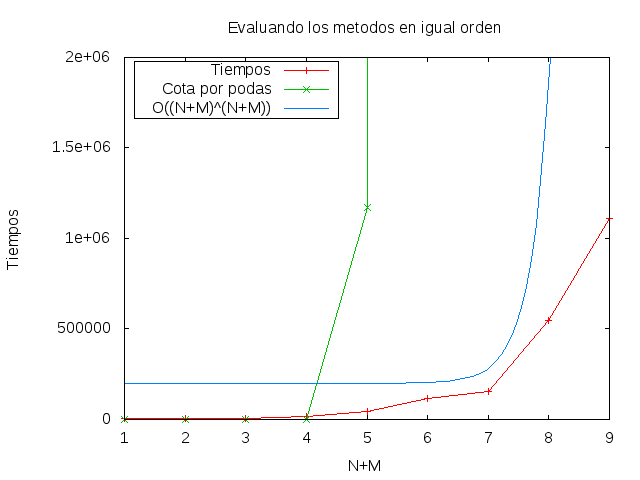
\includegraphics[width=10cm]{./imagenes/tiemposEj1Igual.png}
    \caption{Tiempos evaluando en el mismo orden la forma de enviar personas a la otra orilla}
    %\label{fig:my_label}
\end{figure}

\newpage

En el segundo gráfico podemos observar la diferencia de desempeño entre el algoritmo utilizado en el gráfico anterior, y la versión final del mismo donde la única diferencia es que \textbf{vuelta()} primero evalúa enviar 1 persona a la orilla origen.


\begin{figure}[H]
    \centering
    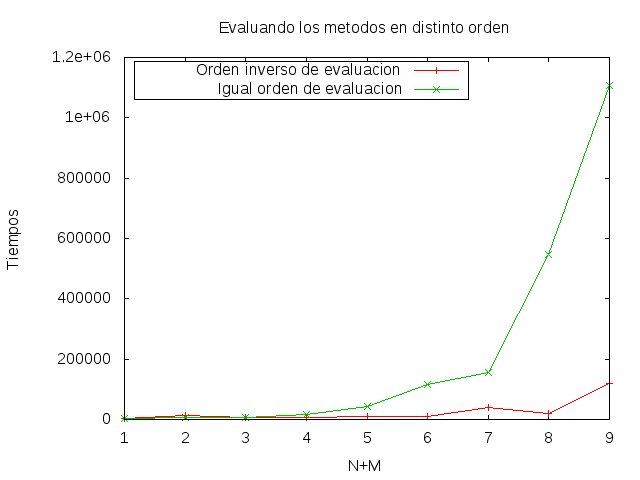
\includegraphics[width=10cm]{./imagenes/tiemposEj1Cambiados.png}
    \caption{Diferencia de tiempos entre evaluar los métodos de la misma forma o discriminar entre ida() y vuelta()}
    %\label{fig:my_label}
\end{figure}

Para mayor detalle, agregamos gráficos fijando N y variando M y viceversa, y los comparamos con los promedios antes tomados.

\begin{figure}[H]
    \centering
    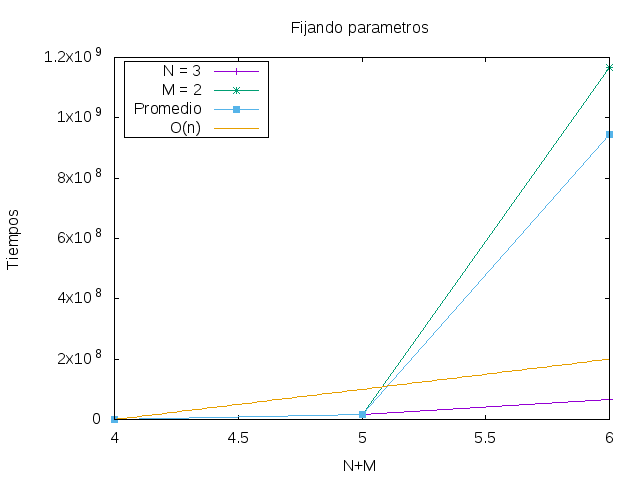
\includegraphics[width=10cm]{./imagenes/fijos.png}
    \caption{Diferencia para un mismo N y M respecto al promedio de todas las combinaciones válidas}
    %\label{fig:my_label}
\end{figure}

Podemos ver como para un mismo N+M, se ve m\'as influyente la cantidad de arque\'ologos que la cantidad de can\'ibales. Entendemos que esto ocurre porque cuando N y M son iguales, las operaciones v\'alidas para los estados son menos que las operaciones v\'alidas cuando N es mayor a M. Y como devolvemos en $\mathcal{O}(1)$ que una operaci\'on no es v\'alida, la curva de N=3 es mucho menor que la curva de M=2
